\documentclass[runningheads]{llncs}
\usepackage[T1]{fontenc}
\usepackage{graphicx}
\usepackage{booktabs}
\usepackage{amsmath}

\begin{document}

\title{Towards Trustworthy and Reliable Deployment of Adversarial Attack Detection for Brain MRI Classification}
\titlerunning{Adversarial Attack Detection for Brain MRI Classification}

\author{Ota Wakabayashi\inst{1} \and Surasak Phetmanee\inst{2,*}\orcidID{0000-0002-8913-1124}}
\authorrunning{O. Wakabayashi and S. Phetmanee}
\institute{National Institute of Technology, Nagano College, Japan\\
\email{22200@g.nagano-nct.ac.jp}
\and
Department of Electrical and Computer Engineering, Faculty of Engineering, Thammasat School of Engineering, Thammasat University, Thailand\\
\email{psurasak@engr.tu.ac.th}}

\maketitle

\begin{abstract}
Adversarial attack detectors are commonly reported using ROC-AUC or
detection rates at a false-positive rate (FPR) calibrated on
training-side data. On a four-class brain-tumor MRI task, we show that
this convention overstates deployed performance: thresholds targeting a
10\% FPR achieve 13.56\% and 15.44\% on the test collection, while
ROC-AUC remains high. Recalibration using 400 clean images from the
deployment collection reduces the evaluation FPR to 10.75\%, without
requiring labelled attacks. At this fixed operating point, an
FGSM-trained detector also detects unseen PGD attacks within two
percentage points of its FGSM performance on identical images. The
reported results were reproduced independently in two Google Colab T4
runs.

\keywords{Adversarial examples \and Attack detection \and Medical
imaging \and Calibration \and False positive rate.}
\end{abstract}

\section{Introduction}

Deep networks for medical image classification are easy to fool with
imperceptible perturbations \cite{goodfellow2015fgsm}, and the
incentives to fool them are concrete in medicine: insurance and billing
fraud, manipulation of imaging endpoints in trials, and sabotage of
automated triage have all been articulated as realistic motivations
\cite{finlayson2019}. A body of work has answered with detectors that
flag adversarial inputs. For
medical imaging the literature's headline is optimistic: adversarial
perturbations distort feature statistics so strongly that simple
detectors reach over 98\% AUC \cite{ma2021understanding}. Yet a detector
is deployed at a \emph{threshold}, not at an AUC, and in a hospital the
cost of a false alarm (a repeated scan, a delayed diagnosis) makes the
achieved false-positive rate a condition of use rather than an
implementation detail.

This paper asks what happens to the operating point between the lab and
deployment, using a brain-tumor MRI classifier as the test bed. Our
contributions:
\begin{enumerate}
\item \textbf{A measured failure of threshold transfer.} On a standard
  Kaggle brain-tumor dataset whose \texttt{Training/} and
  \texttt{Testing/} folders are distinct collections, a detector
  threshold selected for FPR $\le 10\%$ on validation data achieves
  13.6\% on test; a leakage-free calibration split makes it 15.4\%
  (Table~\ref{tab:fpr}). The drift is confined to the upper tail of the
  clean-score distribution, exactly where thresholds operate, while
  ROC-AUC remains high --- so AUC-only reporting cannot reveal the
  operating-point failure.
\item \textbf{A measured remedy.} Calibrating on deployment-side data
  is standard practice; what we contribute is the measurement that, on
  this task, 400 \emph{clean} images from the deployment collection
  reduce the evaluated FPR to 10.75\% (a $+0.75$-point error, compared
  with $+5.44$ points for leakage-free training-side calibration) --- no
  attack examples are needed, matching what a hospital actually has.
\item \textbf{Honest re-pricing, and cross-attack transfer at the pinned
  point.} At the deployment-calibrated 10.75\% FPR, the detection rate
  for successful FGSM attacks is 36.0\% ($\varepsilon=0.01$), 73.4\%
  (0.05), 86.1\% (0.1), and 96.5--98.5\%
  ($\varepsilon \ge 0.25$). Trained on FGSM only, the
  detector detects successful PGD attacks (10 and 40 steps, random
  start) within $\pm$1--3 points of these numbers on the \emph{same}
  images (intersection protocol, Table~\ref{tab:intersection}). All
  paired differences are below two percentage points.
\item \textbf{A strict-dominance observation.} At every $\varepsilon$
  tested, every image broken by FGSM is also broken by PGD
  ($n_{\mathrm{FGSM~only}}=0$ in all 12 pairings) --- direct evidence
  that FGSM-only robustness evaluation is optimistic.
\end{enumerate}

We deliberately label only \emph{successful} attacks (a correct
diagnosis turned incorrect) as positives: unsuccessful perturbations are
noise for a clinical threat model. All experiments run under a pipeline
in which every model artifact is SHA-256-chained and every downstream
stage verifies hashes and clean accuracy before computing.

\section{Related Work}

\textbf{Consistency-based detection.} Feature squeezing
\cite{xu2018squeezing} compares predictions before and after input
squeezing (bit-depth reduction, blur) and thresholds the $L_1$
difference, selecting the threshold on clean data for a target FPR. Our
detector learns from a richer consistency representation (penultimate
features, class probabilities, blur-consistency summaries,
confidence/margin/entropy) but inherits the clean-calibrated-threshold
idea --- and measures what \cite{xu2018squeezing} did not: whether that
threshold survives a collection shift.

\textbf{Detection in medical imaging.} Ma et al.\
\cite{ma2021understanding} established that medical adversarial examples
are easy to detect ($>$98\% AUC on X-ray, fundoscopy, dermoscopy). Our
AUCs agree; our point is that the AUC-to-operating-point gap is where
deployment fails. A DFT-based detector has been proposed for MRI
Alzheimer's classification \cite{dftmri2024}; it labels all adversarial
inputs positive and does not examine FPR transfer.

\textbf{Defense on the same task.} A recent multi-layered defense for
brain tumor classification \cite{scireports2025braintumor} combines
adversarial training with feature squeezing on the same dataset family
--- complementary robustness, not detection; no detector, FPR, or
calibration is involved.

\textbf{Cross-attack generalization.} That detectors trained on one
gradient attack generalize to others is documented in the natural-image
literature; AED-PADA \cite{aedpada2024} improves it further via
multi-source domain adaptation. We therefore do not claim cross-attack
transfer as novel; our contribution is measuring it \emph{at a pinned
deployment operating point} and on an intersection of success sets,
which removes the changing-denominator confound.

\section{Experimental Setup}

\textbf{Task and data.} Four-class brain-tumor MRI classification
(glioma, meningioma, no-tumor, pituitary), 5{,}600 training and 1{,}600
test images (balanced, $224\times224$, pixel range 0--255)
\cite{dataset_needs}. The training folder is split 80/20 into 4{,}480
train / 1{,}120 validation source images with verified zero overlap.

\textbf{Dataset audit.} Because our central claim concerns a shift
between the dataset's two folders, we audited all 7{,}200 images. Three
findings (Table~\ref{tab:audit}). (i)~\emph{Test--train duplication:}
100 of the 400 meningioma test images are pixel-identical, re-encoded
duplicates of Training images (verified by z-normalised downsampled
matching with full-resolution confirmation; 64-bit perceptual hashes
produce false alarms on MRI slices and were not used). Excluding them
\emph{raises} clean accuracy (81.9\% $\to$ 83.6\% overall; meningioma
64.3\% $\to$ 67.0\%), so the contamination does not inflate our
results --- we disclose it rather than correct for it.
(ii)~\emph{Manufactured balance:} the meningioma class in both folders
is padded with synthetic augmentations (100 train / 103 test) to reach
round per-class counts; these synthetic images contain no duplicates.
(iii)~\emph{A banner-marked subpopulation:} many images carry burned-in
text or colour banners from their web sources. Their prevalence differs
sharply between folders for glioma (1.2\% of Training vs.\ 13.3\% of
Testing), and the classifier collapses on exactly that subpopulation:
15.1\% accuracy on banner-flagged glioma test images vs.\ 74.4\% on
unflagged ones --- a reminder that a deployed model can fail almost
completely on an identifiable acquisition subpopulation while aggregate
accuracy looks acceptable. The collection shift behind our FPR finding is thus
concrete and visible in the pixels, not only in detector score
statistics. A shortcut-learning hypothesis for the no-tumor class
(61\% banner prevalence, the classifier's best class) was tested and
refuted: flagged no-tumor images are classified slightly \emph{worse}
($-1.6$ points).

\begin{table}
\centering
\caption{Dataset audit: banner-flagged image prevalence and its effect
on clean test accuracy, per class.}
\label{tab:audit}
\begin{tabular}{lcccc}
\toprule
Class & Flagged (Train) & Flagged (Test) & Acc.\ flagged & Acc.\ unflagged \\
\midrule
Glioma     & 1.2\%  & 13.3\% & 15.1\% & 74.4\% \\
Meningioma & 9.9\%  & 21.5\% & 66.3\% & 63.7\% \\
No tumor   & 62.9\% & 60.5\% & 97.1\% & 98.7\% \\
Pituitary  & 15.7\% & 16.0\% & 98.4\% & 99.1\% \\
\bottomrule
\end{tabular}
\end{table}

\textbf{Classifier.} ImageNet-pretrained MobileNetV2
\cite{sandler2018mobilenetv2}, frozen backbone, light augmentation,
trained head (Adam $10^{-3}$, $\le 10$ epochs, early stopping); clean
test accuracy 81.94\% (1{,}311/1{,}600). This classifier is a testbed
for the calibration question, not a clinical tool --- its accuracy,
particularly on meningioma, is far below any deployable bar. Training is
fully seeded with op determinism, and the canonical model file is never
overwritten --- downstream stages refuse to run if its hash changes.
The reported pipeline was run independently by both authors on Google
Colab Tesla T4 GPUs with TensorFlow 2.20.0 and seed 42; both runs
produced the same evaluation metrics.

\textbf{Attacks.} Untargeted white-box FGSM \cite{goodfellow2015fgsm} on
the 0--255 input scale at $\varepsilon \in \{0.01, 0.05, 0.1, 0.25, 0.5,
1.0\}$\footnote{On the usual $[0,1]$ convention, $\varepsilon=1$ here is
$1/255 \approx 0.0039$ --- small budgets by natural-image standards,
which makes the near-total attack success at $\varepsilon \ge 0.5$ the
more striking.}; PGD \cite{madry2018pgd} with random start, step
$\alpha=\varepsilon/4$, $K \in \{10, 40\}$, with per-batch assertions
keeping every perturbation inside the $\varepsilon$-ball. FGSM at
$\varepsilon=1$ already yields 95.0\% attack success on
initially-correct images; PGD-40 reaches 100.0\% (979/979 on the
evaluation split) --- the undefended classifier offers no robustness at
that budget.

\begin{figure}[t]
\centering
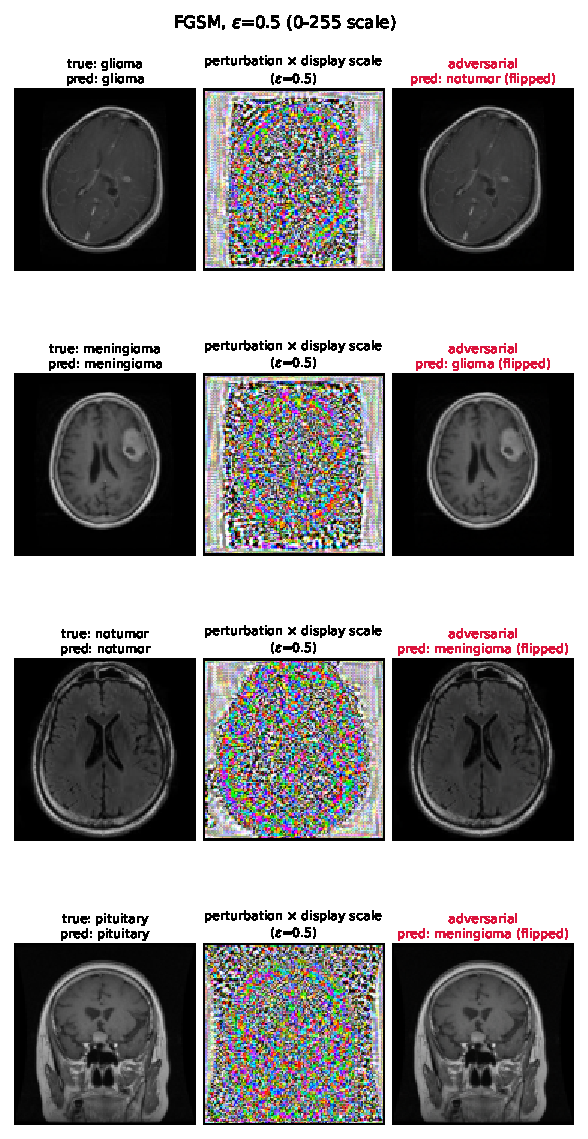
\includegraphics[width=0.42\textwidth]{exp1/fgsm_examples_eps0.5_perclass.pdf}\hfill
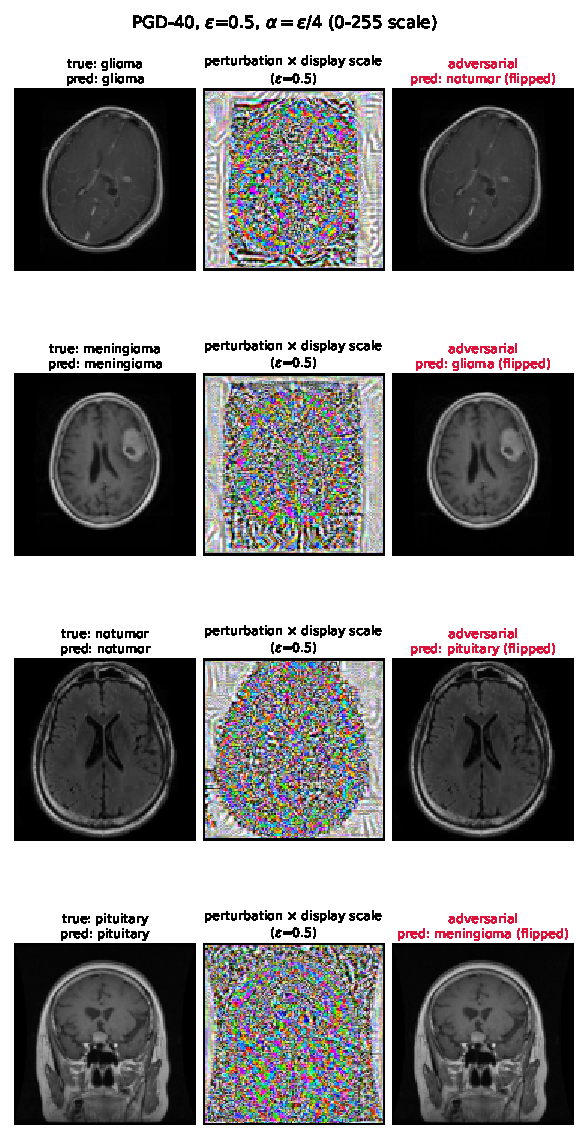
\includegraphics[width=0.42\textwidth]{exp1/pgd40_examples_eps0.5_perclass.pdf}
\caption{One example per class at $\varepsilon=0.5$ under FGSM (left)
and PGD-40 (right): original, perturbation (amplified for display), and
adversarial image with the flipped prediction. The perturbation is
imperceptible at native contrast, yet every diagnosis changes. Exemplars
were screened to exclude banner-marked, synthetic, and duplicated images
(Sect.~3, dataset audit).}
\label{fig:examples}
\end{figure}

\textbf{Detector.} A two-layer MLP (256/64, dropout) on a consistency
feature vector extracted from the \emph{frozen} classifier: penultimate
GAP features, class probabilities before and after a light average-pool
blur, their differences, and confidence/margin/entropy summaries.
Positives are successful attacks only, at training $\varepsilon \in
\{0.01, 0.1, 0.5\}$; class weights balance the loss. Model selection
uses a 560-image validation half (val\_A); the other 560 images
(val\_B) are reserved for threshold calibration and touch neither
training nor selection.

\textbf{Evaluation protocol.} The 1{,}600 test images are split (seeded)
into 400 calibration / 1{,}200 evaluation images. Every reported test
number comes from the 1{,}200 evaluation images at one fixed threshold;
the test set is never used for tuning. $\varepsilon$ values 0.05, 0.25,
1.0 are unseen by the detector.

\textbf{Pipeline integrity.} Security evaluations are unusually
sensitive to silent artifact drift: if the classifier is ever retrained
between the detector-fitting and final-evaluation stages, the test
tables mix incompatible eras without any error being raised. Our
pipeline therefore records the SHA-256 of every trained model in a
manifest together with its clean test accuracy, and every downstream
stage re-verifies both before computing anything, failing closed on
mismatch. Training is fully seeded with deterministic ops, so
two independent Colab T4 executions reproduced the reported evaluation
metrics. Serialized model hashes may differ because of file-level
metadata, so we claim reproducibility of evaluated results rather than
byte-identical model archives. The design was motivated by exactly such a
silent-retrain incident in an earlier iteration of this study.

\section{The Operating Point Does Not Transfer}

Three calibration strategies against one budget (FPR $\le 10\%$):

\begin{table}
\centering
\caption{Claimed vs.\ achieved false-positive rate under three
calibration strategies.}
\label{tab:fpr}
\begin{tabular}{lccc}
\toprule
Calibration data & Claimed FPR & Achieved test FPR & Error \\
\midrule
Validation, 1{,}120 imgs (also used for selection) & $\le 10\%$ & 13.56\% & $+3.56$ \\
val\_B, 560 imgs (leakage-free) & $\le 10\%$ & 15.44\% & $+5.44$ \\
400 clean deployment-collection imgs & $\le 10\%$ & \textbf{10.75\%} & $\mathbf{+0.75}$ \\
\bottomrule
\end{tabular}
\end{table}

\begin{figure}
\centering
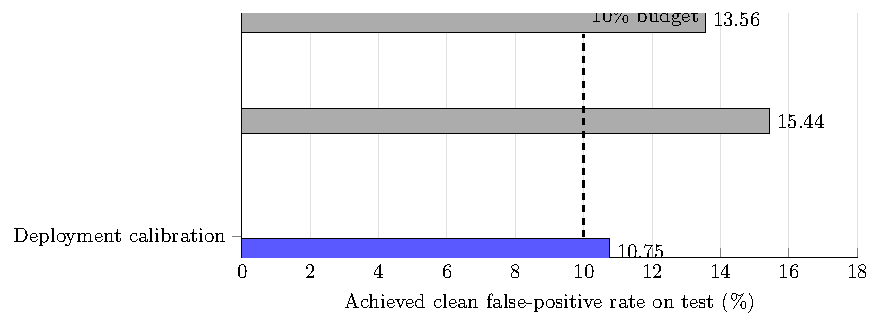
\includegraphics[width=0.55\textwidth]{exp1/fig_fpr_transfer.pdf}
\caption{Achieved clean false-positive rate on the test collection under
the three calibration strategies (budget: 10\%). Deployment-side
calibration comes closest to the target.}
\label{fig:fpr}
\end{figure}

Removing selection leakage (row~2) does not help: the test FPR increases
from the 8.93\% calibration value to 15.44\%. Table~\ref{tab:shift}
shows why. The medians of the full validation and test clean-score
distributions are both near zero, but their upper tails diverge: the
90th percentile increases from 0.189 to 0.351 and the 95th percentile
from 0.400 to 0.687. At the fixed v2b threshold 0.151, the full-split
FPR consequently increases from 10.98\% on validation to 15.44\% on
test. The margin threshold shows the same pattern (9.64\% to 14.25\%).
Because ROC-AUC summarizes score rankings rather than performance at a
fixed threshold, AUC-only reporting cannot reveal this operating-point
failure.

\begin{table}
\centering
\caption{Clean detector-score distributions for the final v2b detector
on the full validation and test splits. The last two columns report the
clean FPR induced by applying the same fixed thresholds to both splits.}
\label{tab:shift}
\begin{tabular}{lcccccc}
\toprule
Split & $p_{50}$ & $p_{75}$ & $p_{90}$ & $p_{95}$ & FPR@0.151 & FPR@0.201 \\
\midrule
Validation ($n{=}1{,}120$) & 0.0001 & 0.0127 & 0.1890 & 0.3996 & 10.98\% & 9.64\% \\
Test ($n{=}1{,}600$)       & 0.0001 & 0.0276 & 0.3514 & 0.6868 & 15.44\% & 14.25\% \\
\bottomrule
\end{tabular}
\end{table}

Calibrating on 400 clean images from the deployment collection lands the
threshold at 0.321, reducing the evaluation FPR to 10.75\%, and requires
no labelled attacks: a
realistic protocol for a hospital that has clean scans but no attack
examples. Deployment-side calibration is standard practice in principle; the
point here is empirical --- how badly the training-side shortcut misses,
and how little data suffices.
Two scoping remarks: the 10\% budget is illustrative (the protocol pins
whatever budget a site chooses; the 7.5\% margin variant behaves
identically), and the calibration set is assumed attack-free --- an
adversary who can poison those 400 images moves the threshold at will,
so their collection must be controlled and auditable.

\textbf{Cost of honesty.} At the pinned threshold, low-$\varepsilon$
detection is lower than the mis-calibrated numbers suggested: 73.4\%
instead of 83.2\% at $\varepsilon=0.05$ (the former on the 1{,}200-image
evaluation subset, the latter on the full test set at its actual 15.4\%
FPR --- the comparison mixes evaluation sets, but both the direction and
the size survive the difference). The earlier figure was bought
with about 54\% more false alarms than the 10\% target.
Table~\ref{tab:deploycal} gives the complete re-priced results. At
$\varepsilon=0.01$, PR-AUC is 0.075 (25 positives vs.\ 1{,}200 cleans):
tiny attacks remain essentially undetectable, and ROC-AUC (0.887)
flatters this regime badly --- we quote PR-AUC alongside ROC-AUC at all
small $\varepsilon$.

\begin{table}
\centering
\caption{Complete FGSM results on the 1{,}200 evaluation images at the
deployment-calibrated operating point (clean FPR 10.75\%). ``Margin'' is
the FPR$\le$7.5\% calibration variant (clean FPR 8.25\%). $\varepsilon$
values marked $\dagger$ were never seen in detector training. The
$\varepsilon=0.01$ row lies below 8-bit input quantization (Sect.~6)
and is reported for completeness only.}
\label{tab:deploycal}
\begin{tabular}{cccccc}
\toprule
$\varepsilon$ & Successful attacks & Detection & Detection (margin) & ROC-AUC & PR-AUC \\
\midrule
0.01           & 25  & 36.0\% & 28.0\% & 0.876 & 0.075 \\
0.05$^\dagger$ & 139 & 73.4\% & 63.3\% & 0.918 & 0.496 \\
0.10           & 310 & 86.1\% & 83.2\% & 0.956 & 0.833 \\
0.25$^\dagger$ & 665 & 96.5\% & 95.8\% & 0.985 & 0.973 \\
0.50           & 865 & 98.3\% & 97.9\% & 0.993 & 0.991 \\
1.00$^\dagger$ & 929 & 98.5\% & 98.3\% & 0.995 & 0.994 \\
\bottomrule
\end{tabular}
\end{table}

\section{Cross-Attack Transfer at the Pinned Operating Point}

Trained on FGSM only, evaluated against PGD it has never seen, at the
same fixed threshold. Table~\ref{tab:pgd} reports the raw PGD results:
PGD is the stronger attack at every $\varepsilon$ (at
$\varepsilon = 1$, PGD-40 breaks all 979 initially-correct evaluation
images), yet detection rates and AUCs remain at FGSM levels. Because PGD
breaks more images than FGSM, raw detection rates have different
denominators; to remove that confound we compare on the intersection of
success sets (Table~\ref{tab:intersection}).

\begin{table}
\centering
\caption{PGD attacks against the FGSM-trained detector at the same
deployment threshold (clean FPR 10.75\%). Attack success is measured on
the 979 initially-correct evaluation images; PR-AUC (not shown) tracks
FGSM's (0.08 at $\varepsilon=0.01$, $\ge 0.56$ from 0.05, $\ge 0.98$
from 0.25). The $\varepsilon=0.01$ rows lie below 8-bit input
quantization and are reported for completeness only.}
\label{tab:pgd}
\begin{tabular}{ccccccc}
\toprule
& \multicolumn{3}{c}{PGD-10} & \multicolumn{3}{c}{PGD-40} \\
$\varepsilon$ & Succ. & Det. & ROC-AUC & Succ. & Det. & ROC-AUC \\
\midrule
0.01 & 2.6\%  & 36.0\% & 0.876 & 2.7\%   & 34.6\% & 0.877 \\
0.05 & 16.9\% & 74.5\% & 0.922 & 17.4\%  & 74.1\% & 0.923 \\
0.10 & 40.6\% & 88.2\% & 0.960 & 41.9\%  & 88.5\% & 0.960 \\
0.25 & 87.1\% & 97.0\% & 0.988 & 89.5\%  & 97.3\% & 0.989 \\
0.50 & 98.6\% & 98.1\% & 0.994 & 99.4\%  & 98.4\% & 0.995 \\
1.00 & 99.9\% & 99.1\% & 0.996 & 100.0\% & 99.0\% & 0.996 \\
\bottomrule
\end{tabular}
\end{table}

\begin{table}
\centering
\caption{Detection rates of successful attacks on the
\emph{intersection} of FGSM and PGD success sets (identical images), at
the deployment-calibrated threshold (clean FPR 10.75\%). The
$\varepsilon=0.01$ row lies below 8-bit input quantization and is
reported for completeness only.}
\label{tab:intersection}
\begin{tabular}{ccccc}
\toprule
$\varepsilon$ & $n$ (intersection) & FGSM & PGD-10 & PGD-40 \\
\midrule
0.01 & 25  & 36.0\% & 36.0\% & 36.0\% \\
0.05 & 139 & 73.4\% & 74.8\% & 74.1\% \\
0.10 & 310 & 86.1\% & 87.7\% & 88.1\% \\
0.25 & 665 & 96.5\% & 96.5\% & 96.7\% \\
0.50 & 865 & 98.3\% & 97.9\% & 98.3\% \\
1.00 & 929 & 98.5\% & 99.0\% & 98.9\% \\
\bottomrule
\end{tabular}
\end{table}

\begin{figure}
\centering
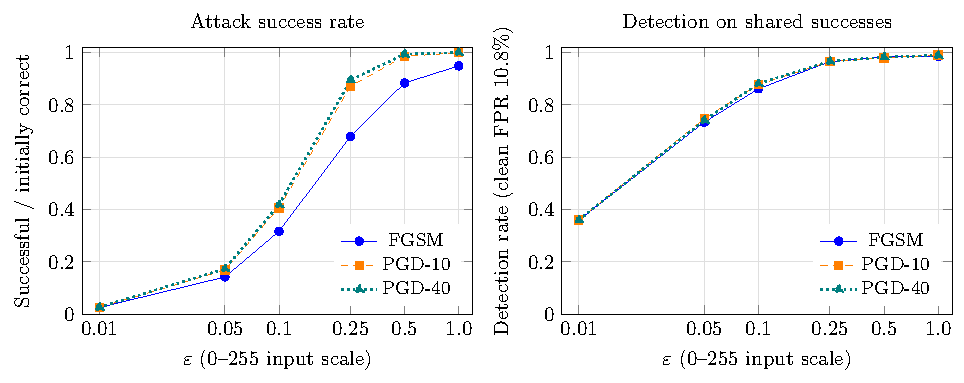
\includegraphics[width=0.88\textwidth]{exp1/fig_attack_detection.pdf}
\caption{Left: attack success rate on initially-correct evaluation
images. Right: detection rate of successful attacks on the intersection
of success sets, at the deployment-calibrated threshold (clean FPR
10.8\%). The detector was trained on FGSM only.}
\label{fig:attackdet}
\end{figure}

On resolution: at these sample sizes the per-row 95\% binomial
half-width is $\approx\pm 1$ point at $p \approx 0.98$
($n = 865$--$929$) and $\pm 7$ points at $n = 139$, so individual row
differences sit at the noise floor; the evidence is consistency of sign
across $\varepsilon$ and both $K$ on paired (identical-image)
comparisons. A paired McNemar-style test from the persisted per-image
scores is future work.

Two observations. \textbf{(1) Transfer holds.} On identical successful
images, every PGD detection rate is within two percentage points of its
FGSM counterpart; ROC-AUC is also nearly identical throughout
(0.876--0.996). The rerun does not support a consistent crossover in
detectability, so we make no claim about the sign of these small paired
differences. \textbf{(2) Strict dominance.}
$n_{\mathrm{FGSM~only}}=0$ in every
pairing: no image at any $\varepsilon$ is broken by FGSM but not by PGD,
so reporting robustness against FGSM alone is provably optimistic on
this task. The images only PGD can break at $\varepsilon \ge 0.25$ are
detected at 98--100\% --- resisting a one-shot attack forces a
perturbation the detector sees clearly.

\textbf{Robustness to the dataset defects.} Excluding the synthetic
meningioma images, the duplicated ones, or both changes every
$\varepsilon \ge 0.1$ intersection entry by about one point or less;
the $\varepsilon = 0.01$ row swings (54\% $\to$ 33\%) purely from its
tiny $n \le 25$. The dataset-defect exclusion analysis was produced with
the original model and is retained as supplementary evidence; it must be
rerun with the final Colab model before its exact FPR values are treated
as part of the primary result set.

\section{Limitations}

$\varepsilon=0.01$ on the 0--255 scale is below one 8-bit quantization
level; FGSM and PGD-10 are nearly identical there, its success
counts are tiny ($n \le 25$), and its detection rate is unstable under
the dataset-exclusion scenarios --- the row is reported for completeness
only. All attacks target the classifier; none optimize to evade the
detector --- a Carlini-style adaptive evaluation is the necessary next
step before any strong defensive claim. The FPR-transfer finding is
measured on one (widely used) dataset whose training/testing split
happens to be a collection split, with one backbone; the audit in
Sect.~3 shows this dataset also carries verbatim test--train duplicates
and synthetic padding, which we disclose and show do not drive our
conclusions, but breadth across cleaner modalities is needed before
generalising. The evaluation set is 75\% of the original test set (400
images are spent on calibration). Per-image scores and masks are
persisted for future paired analyses.

\section{Conclusion}

On a real medical-imaging dataset, the gap between a detector's AUC and
its deployed operating point is where the security claim quietly breaks:
every training-side threshold missed its FPR budget, while 400 clean
deployment images --- no attacks required --- brought it close to the
target. We recommend
that detection papers (i) report the achieved FPR on the evaluation
distribution next to every detection rate, (ii) treat threshold-free
metrics as insufficient for deployment claims, and (iii) compare attack
families on intersections of success sets. Under this stricter
accounting our FGSM-trained consistency detector remains effective
against the non-adaptive attacks evaluated here: at
least 86.1\% detection of successful attacks at $\varepsilon \ge 0.1$
at an achieved clean FPR of 10.75\%, with attack-family differences
below two percentage points on identical images. Whether it survives an adversary that optimizes against the
detector itself is an open question this paper does not answer.

\bibliographystyle{splncs04}
\bibliography{refs}

\end{document}
